\documentstyle[11pt,epsfig,fancybox,semcolor,semlayer,doublespace,portrait]
{seminar}
\input clp_utils

\def\ys{$\Upsilon(1S)$}
\def\yss{$\Upsilon(2S)$}
\def\ysss{$\Upsilon(3S)$}
\def\gamee{$\Gamma_{e^+e^-}$}

% The following strings are needed by the title page and 
% page style definitions in map_utils.tex
\newcommand{\talktitle}[0]{\gamee for \ys, \yss\  and \ysss}
\newcommand{\fmttitle}[0]{}
\newcommand{\conftitle}[0]{April 2002 Meeting of the American Physical Society}
\newcommand{\myname}[0]{Jim Pivarski}
\newcommand{\affila}[0]{Cornell University}
\newcommand{\talkdate}[0]{April 23, 2002}

\pagestyle{conference}   % From clp_utils.tex

% slide magnification
\slidesmag 1

%%%%%%%%%%%%%%%%%%%%%%%%%%%%%%%%%%%%%%%%%%%%%%%%%%%%%%%%%%%%%%%%%%%%%%%%%%%
% Start document
\begin{document}

% Set page size
\slideheight 7.0in
\slidewidth 8.8in 

% Set array stretch
\renewcommand{\arraystretch}{0.3}
\renewcommand{\slidetopmargin}{0.4in}
\renewcommand{\slidebottommargin}{0.9in}


%%%%%%%%%%%%%%%%%%%%%%%%%%%%%%%%%%%%%%%%%%%%%%%%%%%%%%%%%%%%%%%%%%%%%%%%%%%

\begin{slide*}

\slideframe{}
\slideframe*[\dkblue]{Oval}

\begin{center}
\vspace{4 cm}
{\Huge High-precision measurement \\
\vspace{0.25 cm}
of \gamee\  for \ys, \yss\  and \ysss}  \\
\vspace{1 cm}
{\LARGE	Jim Pivarski } \\
% \vspace{0.25 cm}
% {\LARGE	Ritchie Patterson } \\
% \vspace{0.25 cm}
% {\LARGE	Karl Berkelman } \\
\vspace{0.25 cm}
{\Large	(Cornell University) } \\
\vspace{1 cm}
{\LARGE	CLEO Collaboration } \\
\vspace{2 cm}
\conftitle \\
{\large \talkdate}

\end{center}

\end{slide*}

% %%%%%%%%%%%%%%%%%%%%%%%%%%%%%%%%%%%%%%%%%%%%%%%%%%%%%%%%%%%%%%%%%%%%%%%%%%%

% \begin{slide*}

% \slideframe{}
% \slideframe*[\dkblue]{Oval}
% \huge
% \heading{Outline}
% \vspace{1 cm}

% \begin{center}
% \begin{minipage}[t]{12 cm}
% \begin{itemize}
% \LARGE \item {\huge Motivation: verify lattice QCD!}
% \LARGE \item {\huge 2 out of 3 Resonances Scanned}
% \LARGE \item {\huge Energy Calibration Systematics}
% \LARGE \item {\huge Other Systematics / Work to be Done}
% \end{itemize}
% \end{minipage}
% \end{center}

% \end{slide*}
 
%%%%%%%%%%%%%%%%%%%%%%%%%%%%%%%%%%%%%%%%%%%%%%%%%%%%%%%%%%%%%%%%%%%%%%%%%%%

\begin{slide*}

\slideframe{}
\slideframe*[\dkblue]{Oval}
\huge
\heading{Motivation}

\begin{minipage}[t]{\linewidth}
\Large A large contribution to CKM matrix element uncertainties is in
the QCD factors.

\vspace{1 cm}

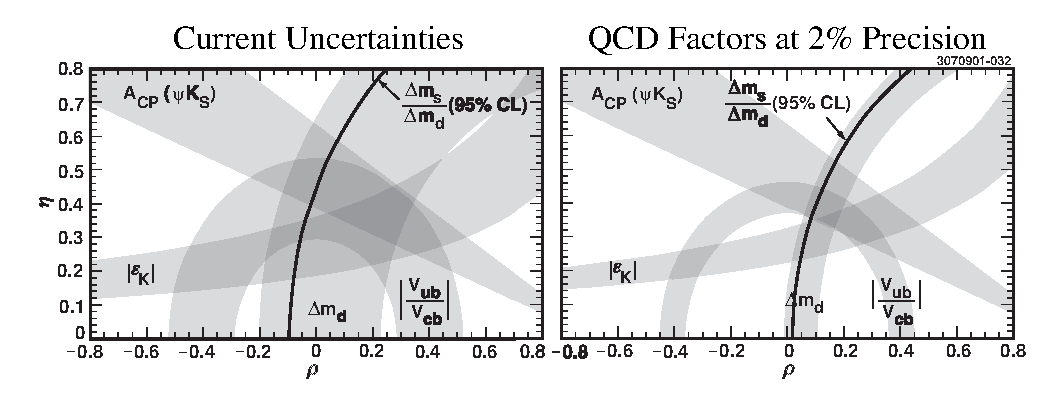
\epsfig{file=theory_errors2.eps, width=\linewidth}

\vspace{1 cm}

Recent improvements to lattice QCD promise to deliver 2\%-level
calculations in the next few years.

\vspace{1 cm}

{\huge But if such high precision results are claimed, on what basis
are they to be believed?}

\end{minipage}

\end{slide*}

%%%%%%%%%%%%%%%%%%%%%%%%%%%%%%%%%%%%%%%%%%%%%%%%%%%%%%%%%%%%%%%%%%%%%%%%%%%

\begin{slide*}

\slideframe{}
\slideframe*[\dkblue]{Oval}
\huge
\heading{Experimental Test of Lattice QCD}

\begin{minipage}[t]{\linewidth}
\Large

$\Gamma(\Upsilon(1S) \to e^+e^-)$, $\Gamma(\Upsilon(2S) \to e^+e^-)$
	and $\Gamma(\Upsilon(3S) \to e^+e^-)$ form three points of
	contact between theory and experiment.

\vspace{0.5 cm}

But the current experimental precisions of 3\%, 5\% and 7\%
	will need to be improved for a tight comparison.

\vspace{1 cm}

{\red \gamee}\  is related to the {\dkblue area under the hadronic cross-section peak}:

\[ {\red \Gamma_{e^+e^-}} = \frac{M_\Upsilon^2}{6 \pi^2}
	\left( 1 + \frac{3}{\frac{1}{\mbox{Br}\{\Upsilon \to l^+l^-\}} - 3} \right)
	{\dkblue \int \sigma_{e^+e^- \to \Upsilon \to {\rm hadrons}} } \]

and can be measured by fitting the resonance peak line-shape.

\vspace{0.5 cm}

\begin{center}
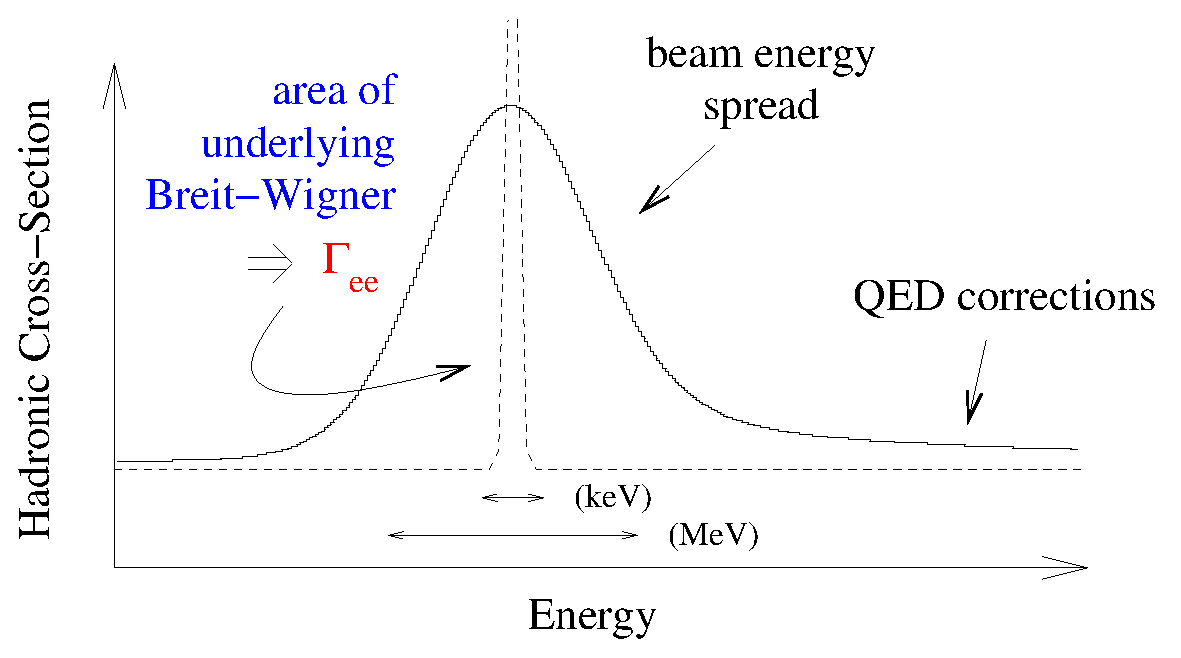
\epsfig{file=cartoon.eps, width=10 cm}
\end{center}

\vspace{0.5 cm}

{ \dkgreen \fbox{ {\LARGE Goal:} To measure \gamee\  for \ys, \yss\  and \ysss\  to $\sim$ 2\%\ldots } }

\end{minipage}

\end{slide*}

%%%%%%%%%%%%%%%%%%%%%%%%%%%%%%%%%%%%%%%%%%%%%%%%%%%%%%%%%%%%%%%%%%%%%%%%%%%

\begin{slide*}

\slideframe{}
\slideframe*[\dkblue]{Oval}
\huge
\heading{Raw Data}

\begin{minipage}[t]{\linewidth}
\Large

{\LARGE Data-taking is complete for the \ys\  and \ysss.}

\vspace{1 cm}

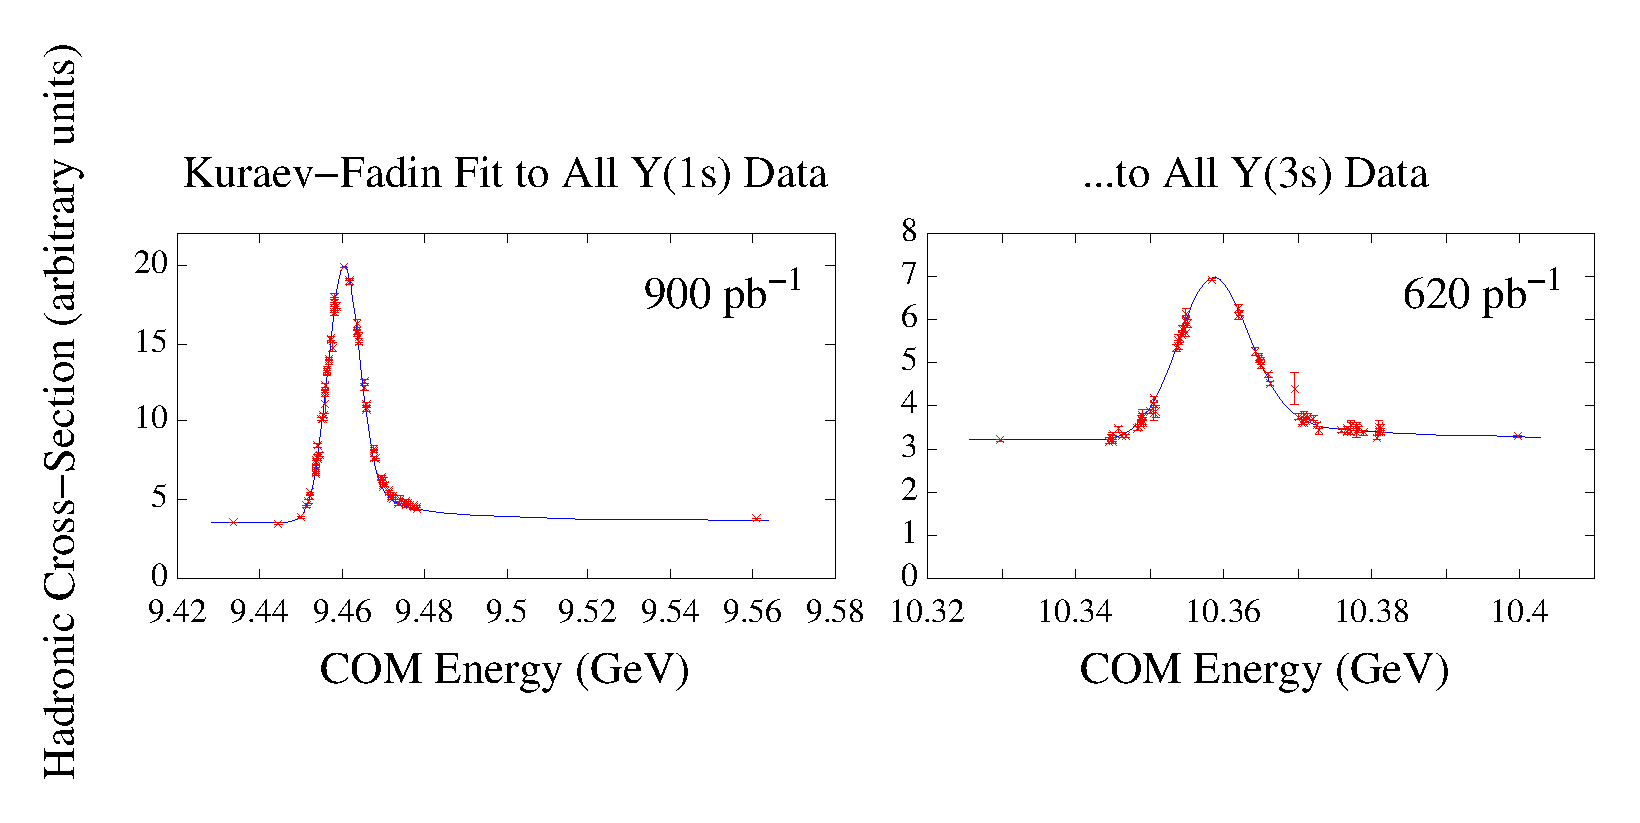
\epsfig{file=fullscans.eps, width=\linewidth}

\vspace{1 cm}

The very high statistics in these scans are to provide for the
opportunity to minimize systematics.

\vspace{1 cm}

Two classes of systematics studies:

\begin{center}
\begin{minipage}[t]{10 cm}
\begin{itemize}
  \LARGE \item energy (horizontal) and
  \LARGE \item efficiency/luminosity (vertical).
\end{itemize}
\end{minipage}
\end{center}

\end{minipage}

\end{slide*}

%%%%%%%%%%%%%%%%%%%%%%%%%%%%%%%%%%%%%%%%%%%%%%%%%%%%%%%%%%%%%%%%%%%%%%%%%%%

\begin{slide*}

\slideframe{}
\slideframe*[\dkblue]{Oval}
\huge
\heading{Energy Systematics}

\begin{minipage}[t]{\linewidth}
\Large

% Effect of energy setting resolution was modeled by Monte Carlo.

% {\large 0.2--0.3 MeV energy fluctuations add 0.5--1\% uncertainty to area
% measurement.}

Protections aganist large-timescale drifts built into scan strategy:

\begin{center}
\begin{minipage}[t]{12 cm}
\begin{itemize}
  \item Scan for each resonance is split up into ten short weekly scans.

  \item Energy point order is randomized.

  \item Each weekly scan begins and ends with the same point, to see
	how well we reproduce the hadronic cross-section there.

\end{itemize}
\end{minipage}
\end{center}

\vspace{1 cm}

Repeated point shows that energy is reproduced to within $\sim$ 0.2 MeV.
Simulations predict that 0.2 MeV RMS fluctuations $\implies$ area
uncertainty of $\sim$ 0.75\%.
\begin{center}
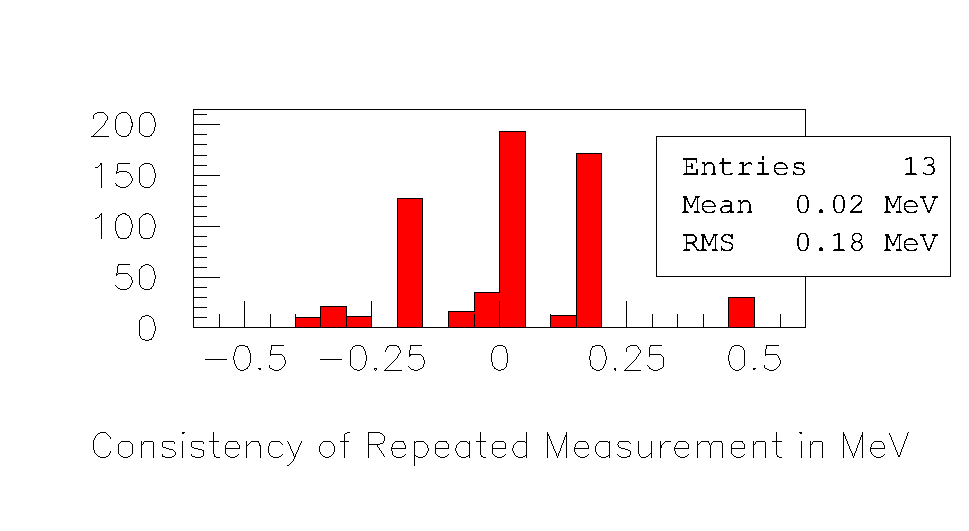
\epsfig{file=consistency2.eps, width=0.7 \linewidth}
\end{center}

% \begin{center}
% \begin{tabular}{c c}
% \begin{minipage}[t]{0.45 \linewidth}
% Repeated point shows that \\
% energy is reproduced to \\
% within $\sim$ 0.3 MeV.
% \end{minipage} &
% \begin{minipage}[t]{0.45 \linewidth}
% 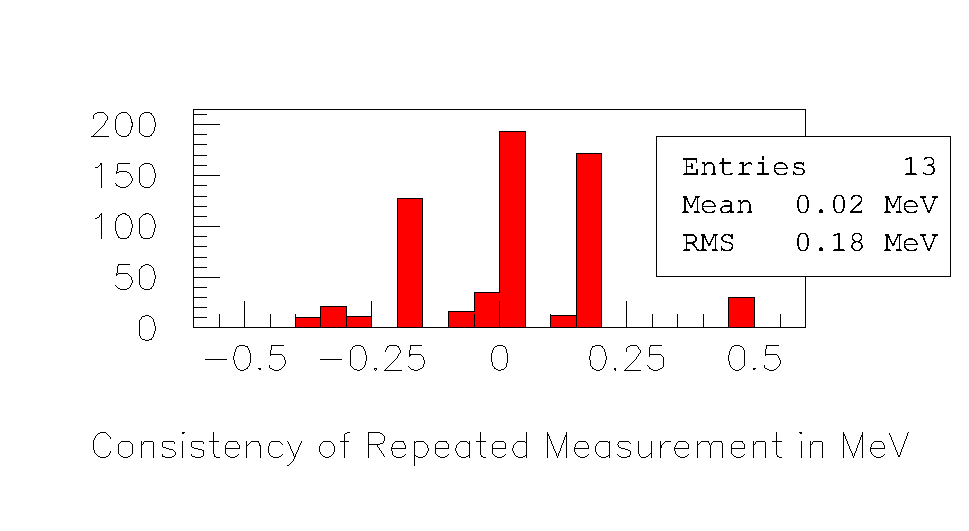
\epsfig{file=consistency2.eps, width=\linewidth}
% \end{minipage}
% \end{tabular}
% \end{center}

Bottom line: the area measurement {\it is} stable.
\begin{center}
\begin{minipage}[t]{12 cm}
\begin{tabular}{r c l}
  std dev area / average area / $\sqrt{\rm N}$ at \ys & = & 0.72 \%    \\
                                               at \ysss & = & 0.39 \%
\end{tabular}
\end{minipage}
\end{center}

\end{minipage}

\end{slide*}

%%%%%%%%%%%%%%%%%%%%%%%%%%%%%%%%%%%%%%%%%%%%%%%%%%%%%%%%%%%%%%%%%%%%%%%%%%%

\begin{slide*}

\slideframe{}
\slideframe*[\dkblue]{Oval}
\huge
\heading{Efficiency/Luminosity Systematics}

\begin{minipage}[t]{\linewidth}

\vspace{1 cm}

{\Huge Studies yet to be done\ldots}

\vspace{0.5 cm}

\begin{center}
\begin{minipage}[t]{12 cm}
\begin{itemize}

  \LARGE \item Event selection cuts need to be defined

  \LARGE \item Efficiency studies of event selection cuts

  \LARGE \item Handle backgrounds due to $\Upsilon \to \tau^+ \tau^-$

  \LARGE \item Efficiency studies of (and improvements to) the luminosity
  measurement

  \LARGE \item Measure trigger efficiency using \\
	\ysss\ $\to$ \yss\ and
	\ysss\  $\to$ \ys\  events

\end{itemize}
\end{minipage}
\end{center}

\vspace{1 cm}

\LARGE

Along the way, we should be able to produce extremely high precision measurements of

\vspace{-0.8 cm}
\begin{center}
\begin{minipage}[t]{0.8 \linewidth}
\begin{tabular}{p{0.27 \linewidth} p{0.27 \linewidth} p{1 cm} p{0.27 \linewidth}}
\Large \[ \frac{\Gamma_{e^+e^-}(\Upsilon(1S))}{\Gamma_{e^+e^-}(\Upsilon(2S))} \mbox{,} \] &
\Large \[ \frac{\Gamma_{e^+e^-}(\Upsilon(2S))}{\Gamma_{e^+e^-}(\Upsilon(3S))} \] &
\Large \[ \mbox{ and } \] &
\Large \[ \frac{\Gamma_{e^+e^-}(\Upsilon(3S))}{\Gamma_{e^+e^-}(\Upsilon(1S))} \mbox{.} \]
\end{tabular}
\end{minipage}
\end{center}

\end{minipage}

\end{slide*}

%%%%%%%%%%%%%%%%%%%%%%%%%%%%%%%%%%%%%%%%%%%%%%%%%%%%%%%%%%%%%%%%%%%%%%%%%%%

\begin{slide*}

\slideframe{}
\slideframe*[\dkblue]{Oval}
\huge
\heading{Conclusion}

\begin{minipage}[t]{\linewidth}
\huge

\vspace{1 cm}

1--2\% experimental measurement of $\Gamma_{e^+e^-}(\Upsilon(nS))$?

\vspace{1 cm}

It will be a lot of work\ldots

\vspace{1 cm}

But the data looks good, and there's no reason to think it's not
possible!

\end{minipage}

\end{slide*}

\end{document}

% %%%%%%%%%%%%%%%%%%%%%%%%%%%%%%%%%%%%%%%%%%%%%%%%%%%%%%%%%%%%%%%%%%%%%%%%%%%

% \begin{slide*}

% \slideframe{}
% \slideframe*[\dkblue]{Oval}
% \huge
% \heading{}

% \begin{minipage}[t]{\linewidth}

% \end{minipage}

% \end{slide*}

